\documentclass[11pt]{article}

\usepackage[margin=1in]{geometry}
\usepackage{amsmath,amssymb}
\usepackage{booktabs}
\usepackage{enumitem}
\usepackage{graphicx}
\usepackage[hidelinks]{hyperref}

\newcommand{\mustar}{\mu^{\ast}}
\newcommand{\EE}{\mathrm{EE}}
\newcommand{\NQP}{N_{\mathrm{QP}}}

\title{Mathematical Meaning of Morris Trajectories, Replicas, and Source
Positions in the Stage-3 QP Screen}
\author{}
\date{July 28, 2026}

\begin{document}
\maketitle

\section{Purpose}

This note defines the quantities appearing in
\path{figures/stage3_screen_results.png}, especially the subtitle
\[
T=128\text{ trajectories}\;\cdot\;
6912\text{ design points}\times
2\text{ replicas}\times
16\text{ source positions}.
\]
The Morris ``trajectory'' is a path through the material-parameter design
space.  It is not a Geant4 particle or phonon trajectory.

\section{Notation}

\begin{table}[ht]
\centering
\begin{tabular}{@{}cl@{}}
\toprule
Symbol & Definition \\
\midrule
$K$ & number of expanded Morris design variables; here $K=53$ \\
$T$ & number of Morris trajectories; here $T=128$ \\
$p$ & number of Morris grid levels; here $p=4$ \\
$L$ & number of design points per trajectory, $L=K+1=54$ \\
$R$ & number of Monte Carlo replicas per design point; here $R=2$ \\
$P$ & number of source positions per replica; here $P=16$ \\
$n_{\mathrm{evt}}$ & primary events per position; here $125{,}000$ \\
$\boldsymbol{\theta}$ & a vector of all $K$ sampled parameters \\
$[a_j,b_j]$ & sampled physical range of parameter $j$ \\
$\NQP_{i r q}$ & QPs from design point $i$, replica $r$, position $q$ \\
$Y_{ir}$ & QP yield per event for replica $r$ at design point $i$ \\
$Y_i$ & replica-averaged QP yield assigned to design point $i$ \\
$\EE_j^{(t)}$ & elementary effect of parameter $j$ in trajectory $t$ \\
$\mu_j$ & mean signed elementary effect of parameter $j$ \\
$\mustar_j$ & mean absolute elementary effect of parameter $j$ \\
$\sigma_j$ & standard deviation of the elementary effects of parameter $j$ \\
\bottomrule
\end{tabular}
\end{table}

\section{Morris trajectories}

\subsection{One-factor-at-a-time path}

A Morris trajectory is an ordered sequence of $K+1$ design points:
\[
\boldsymbol{\theta}^{(t,0)}
\longrightarrow
\boldsymbol{\theta}^{(t,1)}
\longrightarrow\cdots\longrightarrow
\boldsymbol{\theta}^{(t,K)}.
\]
Between consecutive points, exactly one coordinate changes:
\[
\boldsymbol{\theta}^{(t,s+1)}
-
\boldsymbol{\theta}^{(t,s)}
=
\delta_{t,s}\,\mathbf{e}_{j(t,s)},
\]
where $\mathbf{e}_{j}$ is the unit vector for parameter $j$.  The other
$K-1$ coordinates remain fixed during that step.  Every parameter changes
once in each trajectory, so one trajectory supplies one elementary effect
for every parameter.

For this screen,
\[
K=53,\qquad L=K+1=54,\qquad T=128.
\]
Therefore the number of distinct parameter configurations is
\[
N_{\mathrm{design}}
=T(K+1)
=128(53+1)
=6912.
\]
The total number of elementary effects is
\[
N_{\mathrm{EE,total}}=TK=128\times53=6784,
\]
or 128 elementary effects for each parameter.

\subsection{Four-level Morris step}

After normalizing parameter $j$ to the unit interval,
\[
z_j=\frac{\theta_j-a_j}{b_j-a_j},
\]
the four-level grid is based on
\[
\left\{0,\frac13,\frac23,1\right\}.
\]
The conventional Morris step for $p=4$ levels is
\[
\Delta=\frac{p}{2(p-1)}=\frac{4}{6}=\frac23.
\]
The implementation does not assume this value when analyzing the data.  It
reads the actual change from the stored design and divides by the realized
full range.

\section{Response attached to one design point}

\subsection{Sixteen source positions}

For one material configuration $\boldsymbol{\theta}_i$, the simulation uses
$P=16$ lateral source locations.  The locations are generated once from a
scrambled Sobol design and reused for every material configuration.  Let
$\NQP_{irq}$ denote the QPs generated for design point $i$, replica $r$, and
source position $q$.

The 16 source positions are pooled within one replica:
\[
Y_{ir}
=
\frac{\displaystyle\sum_{q=1}^{P}\NQP_{irq}}
{P\,n_{\mathrm{evt}}}.
\]
For the plotted screen,
\[
P\,n_{\mathrm{evt}}
=16\times125{,}000
=2{,}000{,}000
\]
primary events per replica.

The source positions are not additional Morris design points and do not
produce 16 separate bars in the figure.  They form a fixed spatial scenario
set used to estimate the device-averaged response for one material
configuration.  Reusing the same positions prevents a change in source
location from being mistaken for a material-parameter effect.

\subsection{Two replicas}

Each material configuration is evaluated with $R=2$ Monte Carlo replicas.
The replicas have the same material parameters and source-position set but
different replica seed banks.  Stage 3 assigns their mean to the Morris
design point:
\[
Y_i
=
\frac{1}{R}\sum_{r=1}^{R}Y_{ir}
=
\frac{Y_{i1}+Y_{i2}}{2}.
\]
The effective event count represented by $Y_i$ is
\[
R\,P\,n_{\mathrm{evt}}
=2\times16\times125{,}000
=4{,}000{,}000.
\]
The two replica values also expose Monte Carlo variability through their
difference, but two observations alone give a noisy point-specific variance
estimate.

\subsection{Process and event counts}

Every design point requires
\[
R P=2\times16=32
\]
separate Geant4/G4CMP processes.  Consequently, the complete screen contains
\[
6912\times2\times16=221{,}184
\]
sub-runs and
\[
6912\times4{,}000{,}000
=2.7648\times10^{10}
\]
primary events.

One elementary effect compares two endpoints, each evaluated with 32
sub-runs.  Thus its difference is based on 64 sub-runs and $8\times10^6$
primary events.  Endpoints are shared by neighboring steps of a trajectory,
so they are not rerun separately for each parameter.

\section{Elementary effects and Morris indices}

Suppose parameter $j$ changes between two consecutive points in trajectory
$t$.  Let their responses be $Y_{t,-}$ and $Y_{t,+}$ and their parameter
values be $\theta_{j,t,-}$ and $\theta_{j,t,+}$.  The stage-3 implementation
uses the dimensionless elementary effect
\[
\EE_j^{(t)}
=
\frac{
\left(Y_{t,+}-Y_{t,-}\right)/\overline{Y}
}{
\left(\theta_{j,t,+}-\theta_{j,t,-}\right)/(b_j-a_j)
},
\]
where
\[
\overline{Y}
=
\frac{1}{N_{\mathrm{design}}}
\sum_{i=1}^{N_{\mathrm{design}}}Y_i.
\]
For a normalized four-level Morris step of magnitude $2/3$,
\[
\EE_j^{(t)}
\simeq
\frac{3}{2}
\frac{Y_{t,+}-Y_{t,-}}{\overline{Y}},
\]
with the sign also determined by whether the Morris step moves upward or
downward in parameter $j$.

The signed mean is
\[
\mu_j
=
\frac1T\sum_{t=1}^{T}\EE_j^{(t)}.
\]
Opposite-signed effects can cancel in $\mu_j$, so screening normally uses
\[
\mustar_j
=
\frac1T\sum_{t=1}^{T}\left|\EE_j^{(t)}\right|.
\]
The spread is
\[
\sigma_j
=
\sqrt{
\frac{1}{T-1}
\sum_{t=1}^{T}
\left(\EE_j^{(t)}-\mu_j\right)^2
}.
\]

Interpretation:
\begin{itemize}[leftmargin=*]
\item Large $\mustar_j$: parameter $j$ has a large overall influence on QP
yield over its selected range.
\item Small $\mustar_j$: its effect is weak or indistinguishable from the
simulation noise at this fidelity.
\item Large $\sigma_j$: the effect changes with the other parameters, is
nonlinear, or contains appreciable Monte Carlo noise.
\item Small $\sigma_j$: the effect is comparatively consistent across the
design box.
\end{itemize}

Because the denominator scales the observed step to the full parameter
range, $\mustar_j$ is a normalized full-range slope estimate.  It is not a
literal endpoint-to-endpoint change when the model is nonlinear, and it
depends on the selected parameter bounds.

\section{Meaning of the three figure panels}

\begin{enumerate}[label=\textbf{Panel \Alph*:},leftmargin=*]
\item The horizontal bar is $\mustar_j$.  The horizontal error bar is the
5th--95th percentile bootstrap interval for $\mustar_j$, which is a
two-sided 90\% interval.  The orange dashed line is the dummy-calibrated
noise threshold.
\item This is a separate noise-floor run containing 200 physically identical
configurations.  Each histogram entry pools 16 positions with 250,000 events
per position and one replica:
\[
16\times250{,}000=4{,}000{,}000
\]
events per histogram entry.  It is not the distribution of the two replicas
from the full Morris screen.
\item The horizontal coordinate is $\mustar_j$ and the vertical coordinate is
$\sigma_j$.  Moving right means greater overall influence; moving upward
means greater nonlinearity, interaction, or variability.
\end{enumerate}

\begin{figure}[ht]
\centering
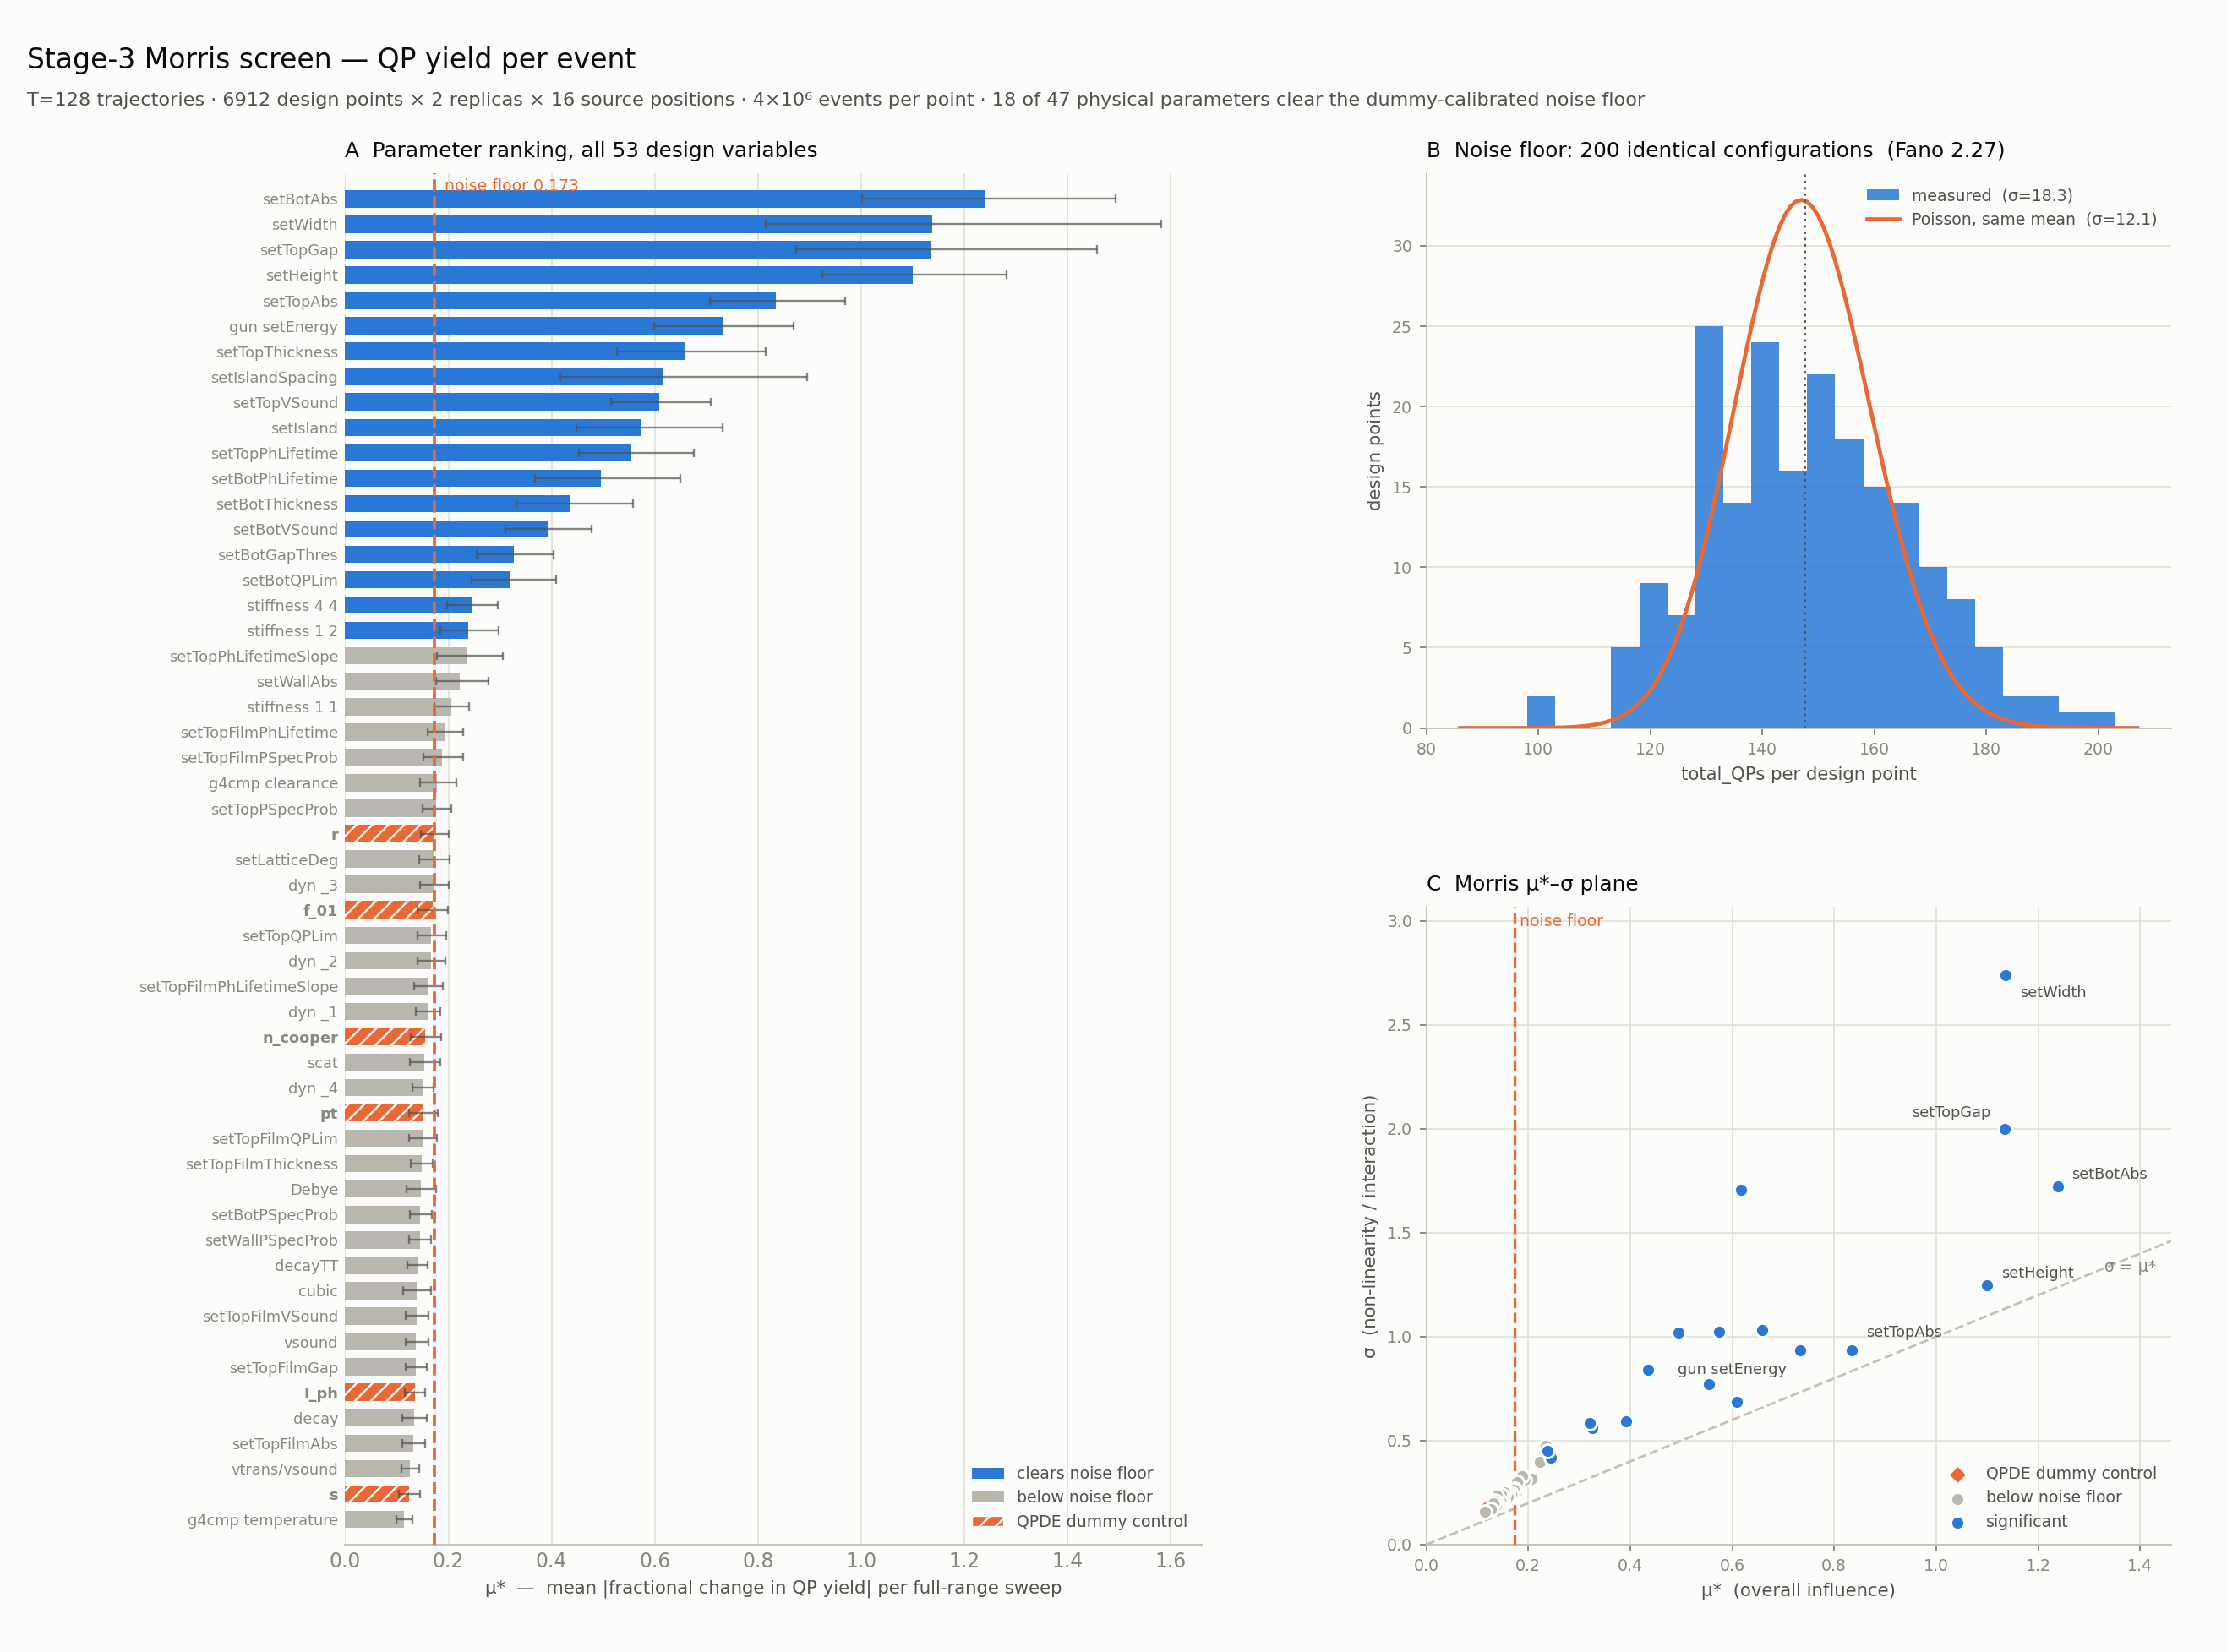
\includegraphics[width=\textwidth]{figures/stage3_screen_results.png}
\caption{Stage-3 Morris screening figure to which the definitions in this
note apply.}
\end{figure}

\section{Mapping to the code}

The stage-1 design is generated conceptually by
\begin{verbatim}
morris_samp.sample(setup, 128, num_levels=4, seed=MORRIS_SEED)
\end{verbatim}
in \path{stage1_run_simulations.py}.  Stage 1 generates
$R\times P$ macros and processes for each design point.

Stage 2 pools the $P=16$ hits files inside each replica and writes one
\path{qp_summary.csv} row per pair $(i,r)$.

Stage 3 performs
\begin{verbatim}
groupby("design_point")[objective].mean()
\end{verbatim}
to obtain $Y_i$, divides the design into consecutive blocks of $K+1=54$
rows, finds the single changed coordinate at every step, and calculates
$\EE_j^{(t)}$, $\mustar_j$, and $\sigma_j$.

\section{Random-seed scope}

The run underlying the current figure was produced before explicit seed
control was added.  Its two replica processes were intended to be independent,
but the later audit found repeated streams from the old
\texttt{clock()}-based initialization.

The current stage-1 code corrects this with explicit CLHEP seeds.  The seed is
a function of
\[
(\text{trajectory},\text{replica},\text{source position})
\]
and not of the step within a trajectory.  Hence the two endpoints of an
elementary effect use the same random stream for a fixed replica and source
position, implementing common random numbers.  Different replicas and
trajectories receive different streams.  Final candidates should still be
validated with a fresh seed bank.

\section{Compact summary}

\[
\boxed{
\begin{aligned}
K&=53, & T&=128, & N_{\mathrm{design}}&=T(K+1)=6912,\\
R&=2,  & P&=16,  & n_{\mathrm{evt}}&=125{,}000,\\
N_{\mathrm{subruns}}&=N_{\mathrm{design}}RP=221{,}184,\\
N_{\mathrm{events/point}}&=RPn_{\mathrm{evt}}=4\times10^6.
\end{aligned}}
\]

Thus, 128 Morris paths explore the 53-dimensional parameter box.  Every one
of their 6,912 material configurations is evaluated by averaging two
replicas, each pooled over the same 16 source locations.

\end{document}
